\documentclass[10pt,twocolumn]{article}

\usepackage[margin=0.75in]{geometry}
\usepackage{amsmath,amssymb}
\usepackage{booktabs}
\usepackage{graphicx}
\usepackage{hyperref}
\usepackage[numbers,sort&compress]{natbib}
\usepackage{microtype}

\title{Proxy-Resistant Benchmarks for Causally Grounded Finite Agents}
\author{Anonymous Authors}
\date{}

\begin{document}
\maketitle

\begin{abstract}
Agent benchmarks often reward final task success, but final success can be
proxy-supported: a model may exploit shortcuts, stale confidence, local final
cues, uniform memory, or brittle tool surfaces. We propose a finite-agent
benchmark design rule: a suite passes only when behavior, a suite-specific
causal/structure gate, and anti-cheat controls all pass. We instantiate the rule
with two hardened anchors. Suite C tests adaptive inquiry under world change:
agents must remain quiet when stable, re-engage after change, recover
attribution, avoid false calm, spend fewer probes than high-cost controls, and
reopen after a second shift. Suite D/E tests long-horizon commitment: a
future-critical variable must survive memory, generated action, tool schema,
repair, causal readout, and black-box API behavior surfaces. The benchmark is
not a consciousness test or production reliability certificate. It is a
controlled diagnostic package for asking whether finite agents succeed for the
right causal reason.
\end{abstract}

\section{Introduction}

Language-agent systems increasingly combine reasoning traces, external actions,
memory, tools, search, and feedback \citep{yao2022react, shinn2023reflexion,
wang2023voyager, ahn2022saycan, yao2023tree}. End-to-end benchmarks evaluate
whether these systems solve tasks in web, OS, software, and general-assistant
settings \citep{liu2023agentbench, zhou2023webarena, xie2024osworld,
mialon2023gaia, jimenez2024swebench}. These benchmarks are valuable, but final
success alone cannot answer a different question: did the agent succeed because
the future-relevant variable was represented, attributed, queried, and committed
at the surface where action was selected?

This paper packages a family of finite diagnostic suites around one minimum pass
rule:
\begin{center}
\fbox{\parbox{0.92\linewidth}{A suite passes only if behavior passes, the
relevant structure gate passes, and anti-cheat controls pass.}}
\end{center}

The rule is motivated by familiar safety and robustness failures. Reward hacking
and specification gaming show that optimizing a measured score can satisfy the
literal metric while missing the intended outcome \citep{amodei2016concrete}.
Goal misgeneralization shows that agents can retain capabilities while pursuing
the wrong objective out of distribution \citep{langosco2022goal}. In
benchmarks, the analogous failure is behavior-only success: the final answer is
right, but the reason is wrong.

\section{Benchmark Design}

Each suite reports a vector score rather than a single leaderboard scalar:
behavior, causal representation, attribution, inquiry, commitment, and
generalization. The axis is included only when the suite can audit it.

\begin{table*}[t]
\centering
\small
\begin{tabular}{p{0.16\linewidth}p{0.34\linewidth}p{0.36\linewidth}}
\toprule
Axis & Question & Example metric \\
\midrule
Behavior & Does it solve the task? & final accuracy, return \\
Representation & Is the right variable tracked? & specificity, patch effect \\
Attribution & Is source assigned correctly? & self/world MAE \\
Inquiry & Does it ask when stale? & re-engagement, probe cost \\
Commitment & Does memory reach action? & tool field, repair value \\
Generalization & Does structure transfer? & compatibility, wrong group \\
\bottomrule
\end{tabular}
\caption{Vector score axes. The benchmark avoids collapsing distinct evidence
types into one scalar.}
\label{tab:axes}
\end{table*}

\paragraph{Anti-cheat controls.}
Controls are suite-specific: matched distractors for memory, visible-control
nulls for shortcut final cues, wrong-group transformations for OOD, shuffled
source labels for attribution, signal suppression for false calm, matched-random
probe budgets for inquiry, and repair/no-op controls for tool commitment.

\section{Suite C: Re-Engagement Under World Change}

Suite C tests whether an agent can reopen inquiry after its world model becomes
stale. The finite harness contains two shifts. The first shift tests
re-engagement after learned quiet; the second tests reopenability after a prior
recovery.

The hand-policy terminal run passes all six gates. The headline
\texttt{burst\_then\_refractory} condition reaches final affected MAE 0.112,
first-shift selectivity 16.927, second-shift reopenability 16.667, and uses
22.6 probes. The matched scheduled and oracle references use 144.0 and 69.5
probes respectively. The false-calm control
\texttt{fixed\_surprise\_decrement} looks quiet but fails recovery with final
MAE 0.517.

The learned-transfer run trains a small probe head from teacher traces and
evaluates it on held-out seeds. The learned head reaches final affected MAE
0.112, first-shift selectivity 16.667, second-shift reopenability 17.448, and
uses 23.1 probes. Stale-signal, wrong-signal, signal-suppression, and
matched-random controls fail in their intended ways.

\begin{figure}[t]
\centering
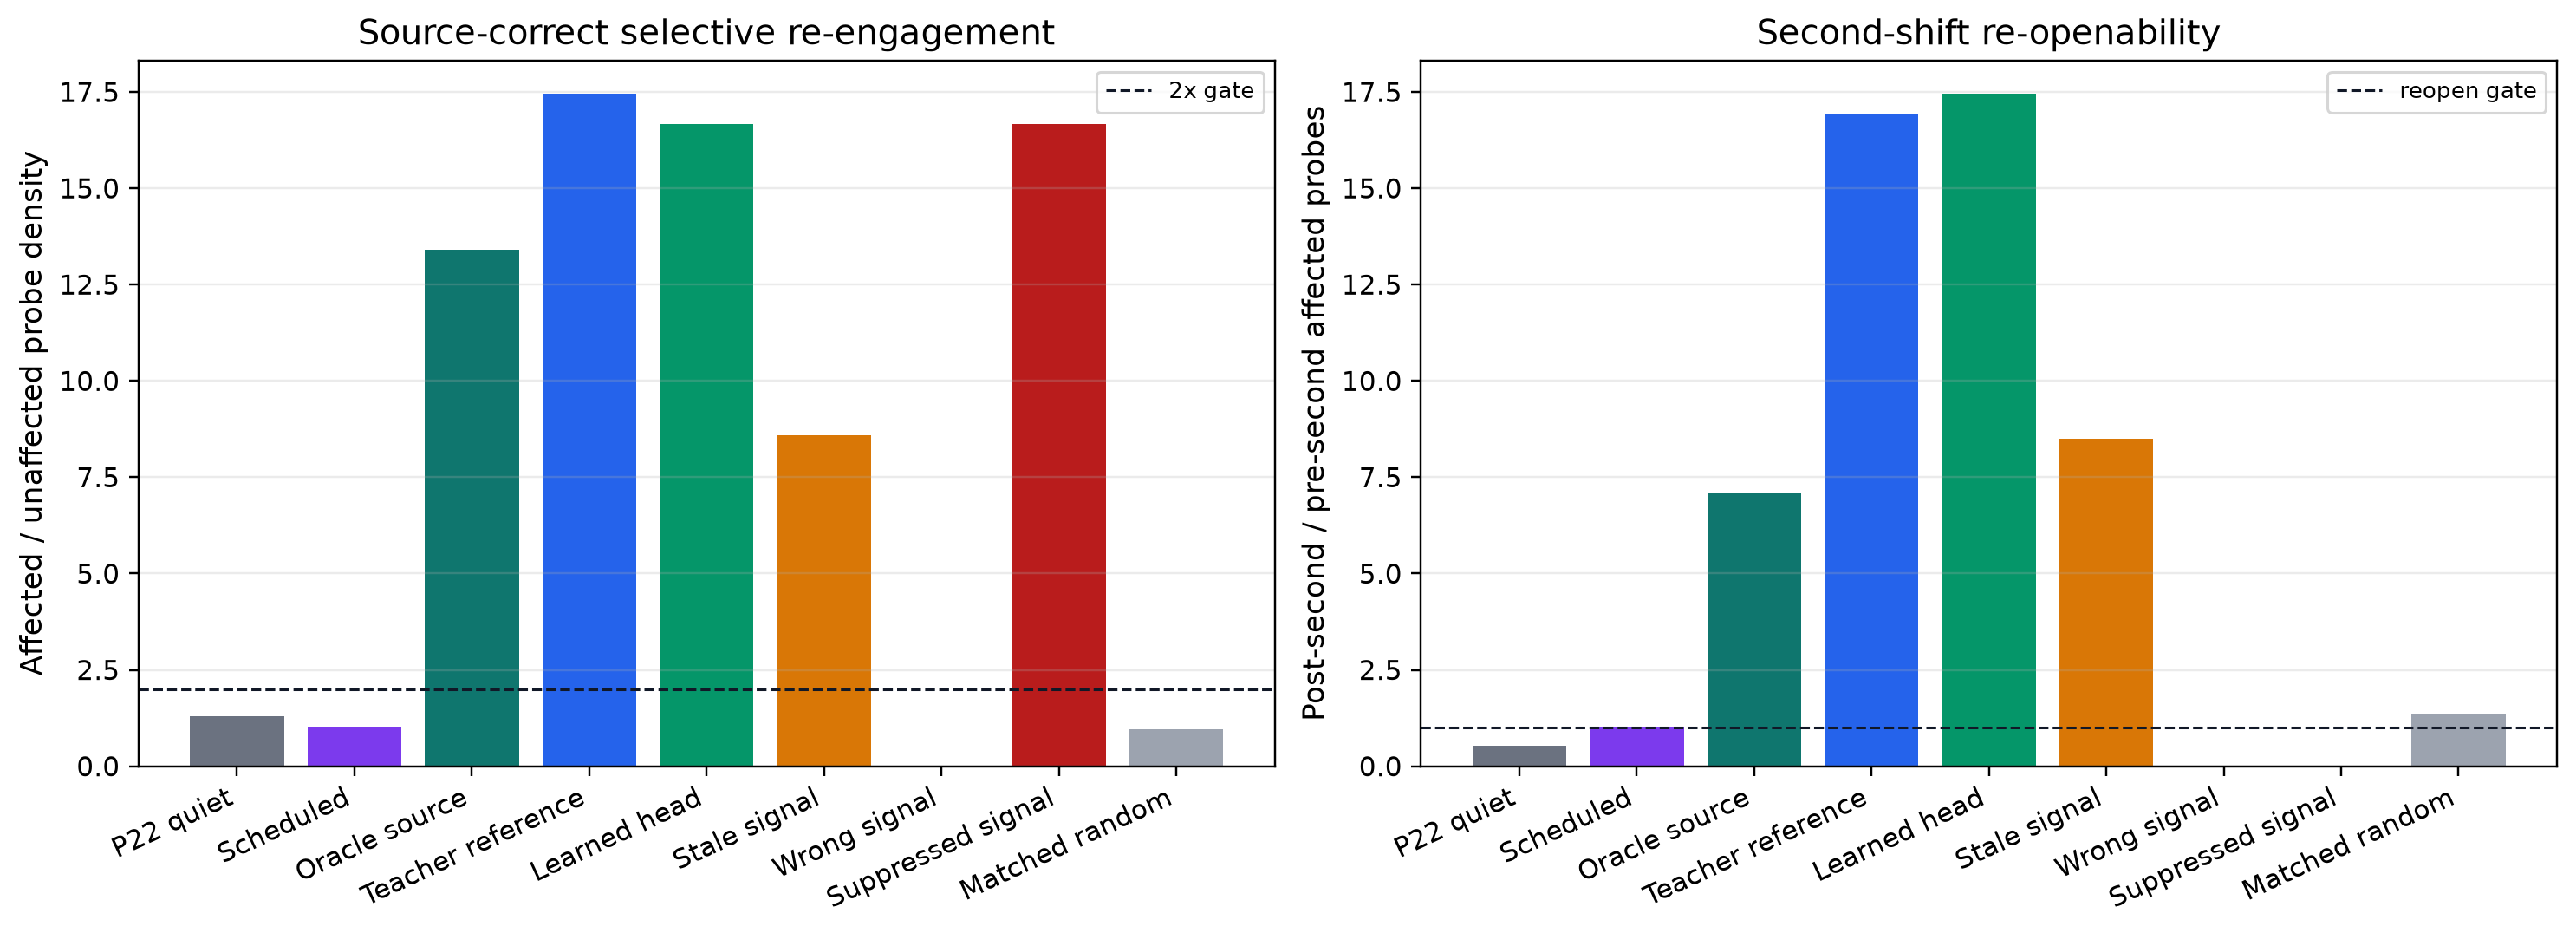
\includegraphics[width=\linewidth]{../../habituated_reengagement/figures/suite_c_neural_fig2_selectivity_reopenability.png}
\caption{Suite C learned-transfer inquiry metrics. The learned head reopens
after both shifts while matched random and wrong-source controls fail.}
\label{fig:suitec}
\end{figure}

\section{Suite D/E: Commitment-Surface Memory}

Suite D/E tests a temporal complement: an early variable matters when it controls
a future action or tool surface. The benchmark moves the future-critical slot
across runs and asks whether memory sensitivity follows that moved bottleneck
rather than matched distractors.

The evidence ladder includes synthetic trained agents, tool commitment, repair
branches, generated JSON-like actions, prompt-level open-model behavior,
hidden-state localization, fixed-action counterfactuals, causal patching,
prompt-family robustness, and black-box API behavior. The strongest
interpretation is not "the model remembers everything." It is the
commitment-surface law: memory becomes agent-relevant when it survives the
interface where it must control action.

\begin{figure}[t]
\centering
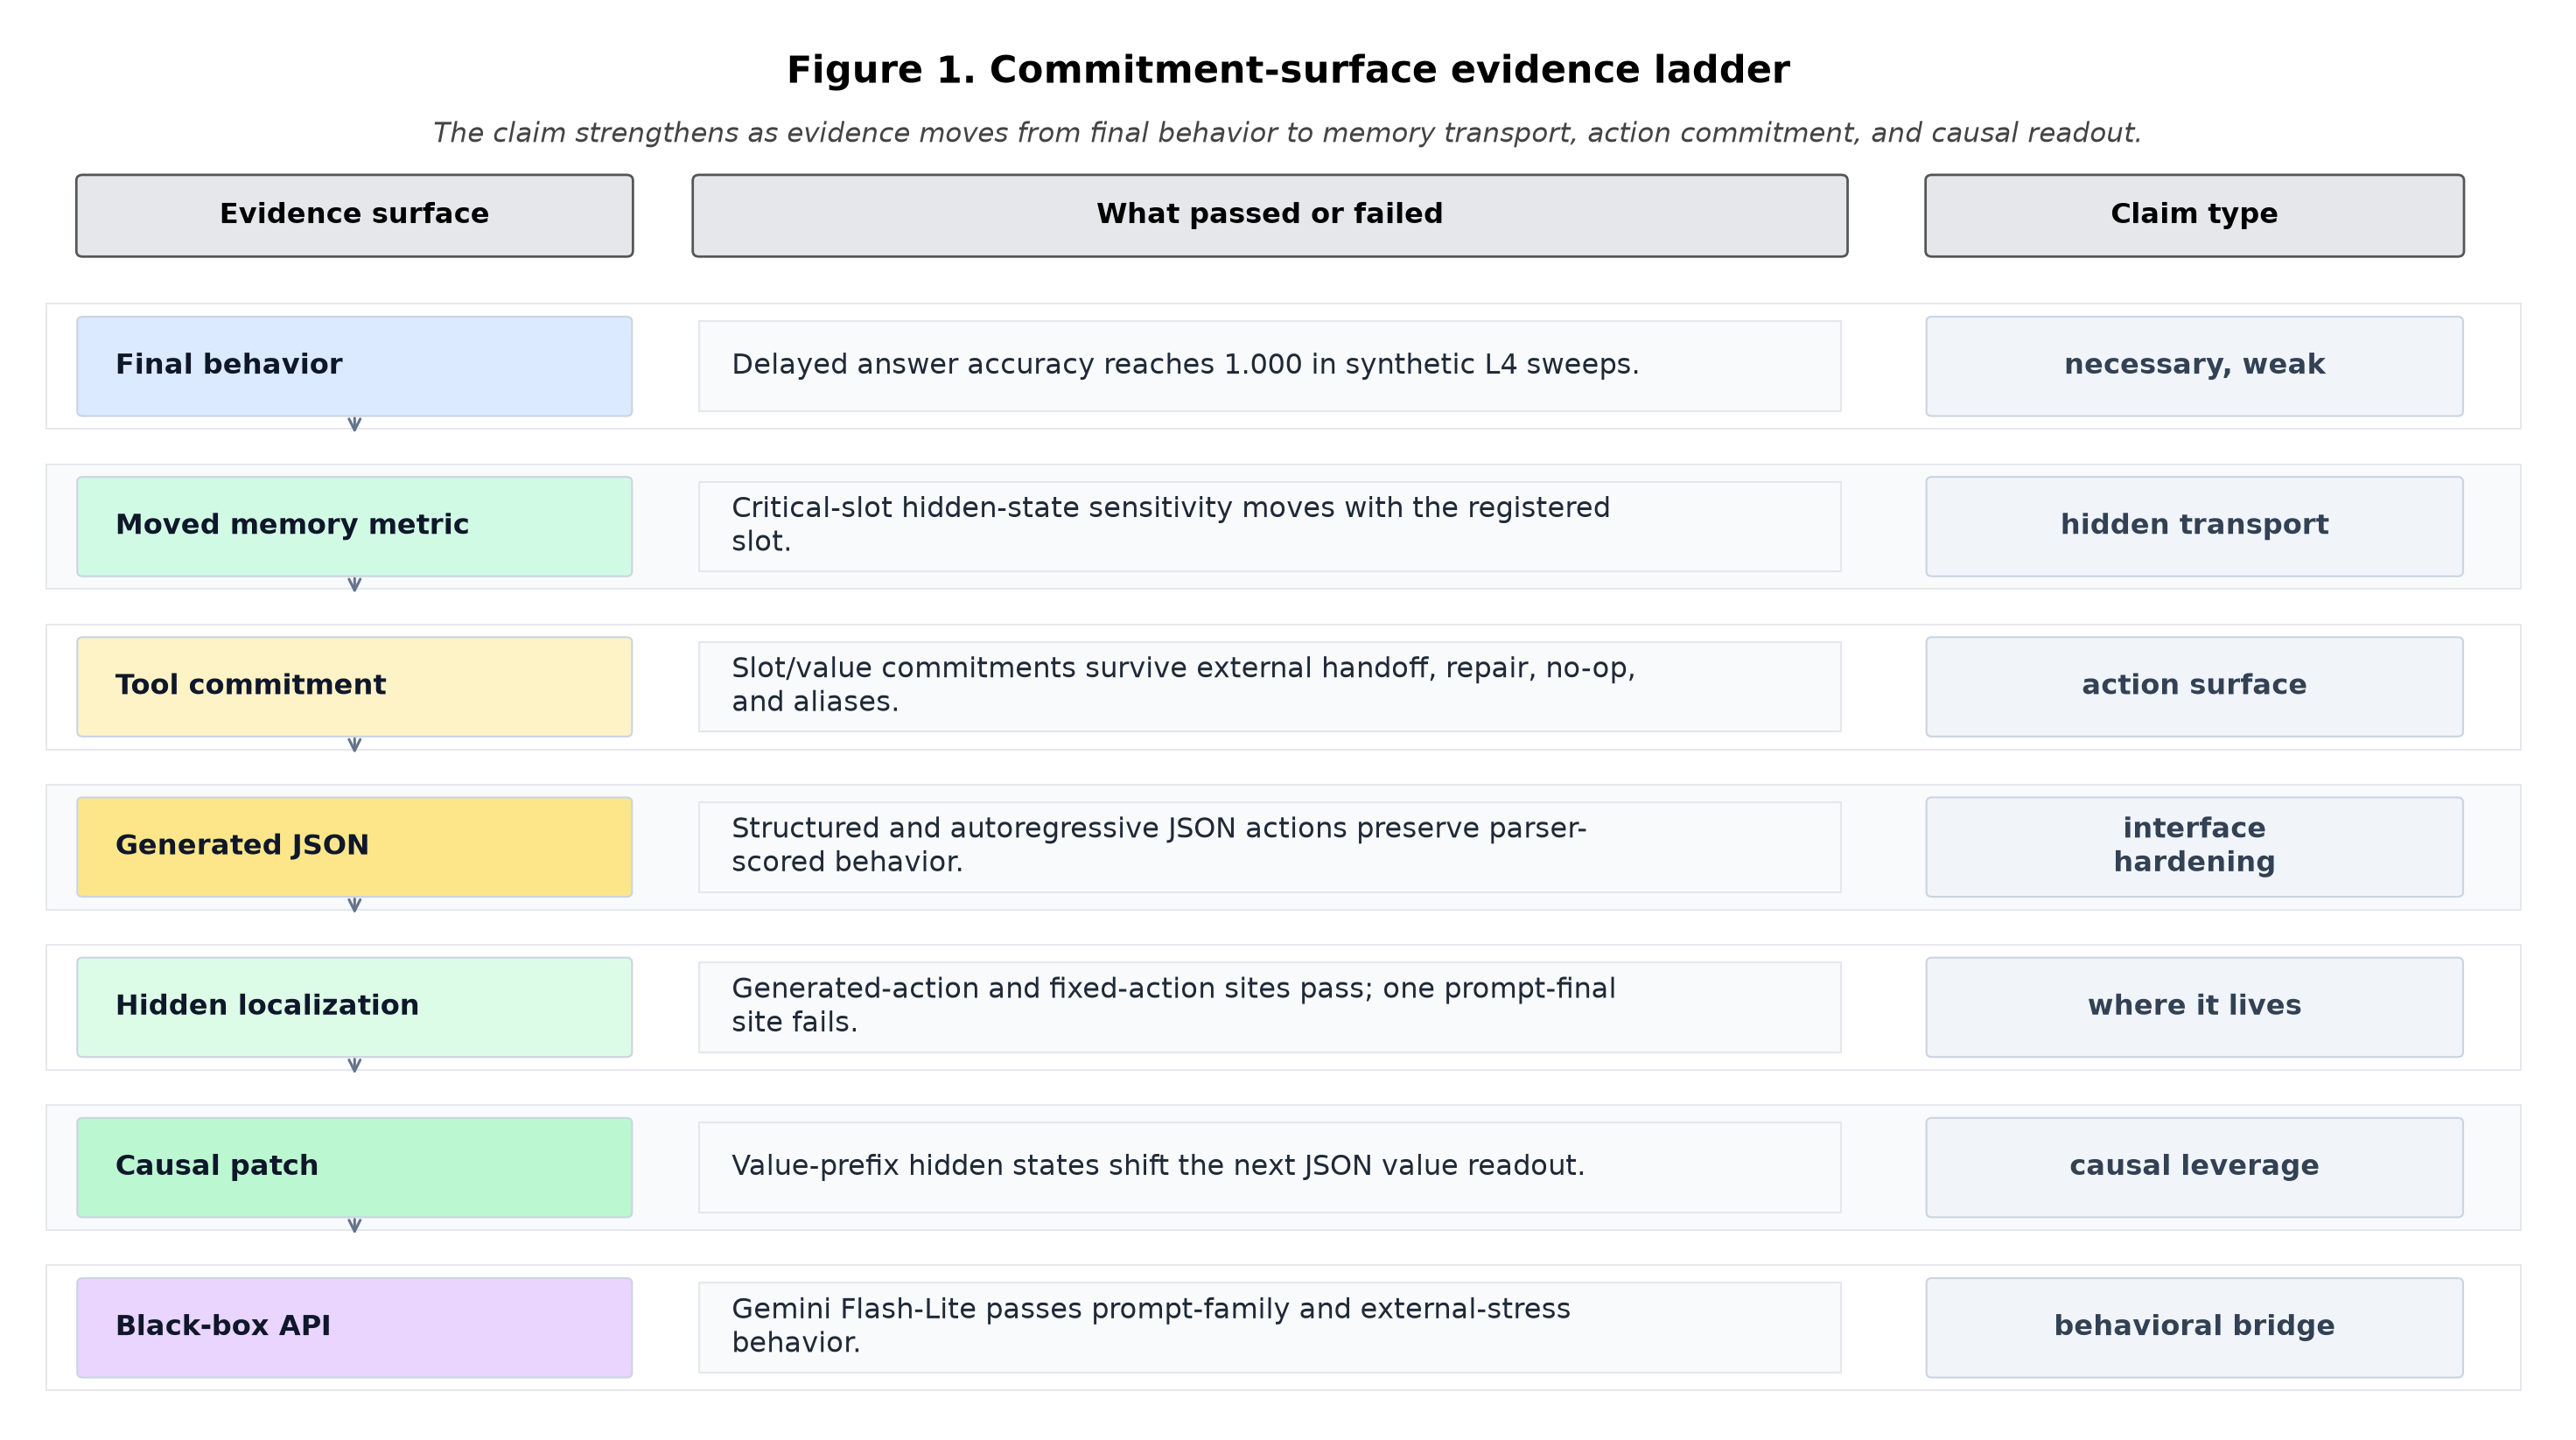
\includegraphics[width=\linewidth]{../../long_horizon_bottleneck/figures/fig1_commitment_surface_ladder.png}
\caption{Commitment-surface evidence ladder. The claim strengthens when the
future-critical variable survives behavior, hidden state, generated action,
repair, causal readout, and API surfaces.}
\label{fig:commitment}
\end{figure}

\section{Release Contract}

A public benchmark release should include task generators, fixed seeds,
declarative manifests, JSONL rows, summary JSON, benchmark cards, lower and
upper baselines, anti-cheat controls, and figure regeneration scripts. The
shared schema requires a benchmark block, suite block, run metadata, minimum
pass rule, score axes, gates, baselines, artifacts, allowed claim, and
non-claims.

\section{Related Work}

The benchmark complements agent mechanisms such as ReAct, Reflexion, Voyager,
SayCan, Toolformer, and Tree of Thoughts \citep{yao2022react,
shinn2023reflexion, wang2023voyager, ahn2022saycan, schick2023toolformer,
yao2023tree}. It also complements end-to-end evaluations such as AgentBench,
WebArena, OSWorld, GAIA, SWE-bench, HELM, and BIG-bench
\citep{liu2023agentbench, zhou2023webarena, xie2024osworld, mialon2023gaia,
jimenez2024swebench, liang2022helm, srivastava2022bigbench}. Our contribution
is narrower: finite diagnostic suites that reveal whether success is supported
by the intended causal structure.

\section{Limitations}

The current suites are finite and controlled. Suite C's learned head is
teacher-trained, not reward-trained or open-agent learned. Suite D/E black-box
API runs are behavioral and do not establish hidden-state localization for
closed models. Synthetic JSON/tool ladders do not certify autonomous
natural-language tool reliability. The benchmark does not test consciousness,
human cognition, biological agency, or production safety.

\section{Conclusion}

Proxy-resistant benchmarking changes the pass condition. Final behavior is
necessary but not sufficient. A finite agent should pass only when the
future-relevant structure reaches the prediction, attribution, inquiry, memory,
or commitment surface where action is chosen, and when anti-cheat controls rule
out the shortcut.

\bibliographystyle{plainnat}
\bibliography{references}

\clearpage
\onecolumn
\appendix
\section{Suite Inventory}

The full benchmark family has six suites:
\begin{itemize}
  \item Suite A: consequence-to-action.
  \item Suite B: reafferent source attribution.
  \item Suite C: re-engagement under world change.
  \item Suite D: long-horizon moved bottleneck.
  \item Suite E: tool commitment and repair.
  \item Suite F: structure-compatible OOD.
\end{itemize}

The main paper centers Suite C and Suite D/E because they are the strongest
current anchors. Suites A/B/F should remain in appendix or a suite-family
overview unless expanded into their own benchmark cards.

\section{Suite C Gate Definitions}

Source:
\path{experiments/world_responds/results/suite_c_reengagement_2026_07_06.md}
and
\path{experiments/world_responds/results/suite_c_neural_transfer_2026_07_06.md}.

\begin{table*}[h]
\centering
\small
\begin{tabular}{lll}
\toprule
Gate & Meaning & Current status \\
\midrule
C1 & baseline silence replication & pass \\
C2 & selective first-shift re-engagement & pass \\
C3 & affected-component recovery & pass \\
C4 & no false calm & pass \\
C5 & cost-aware inquiry & pass \\
C6 & second-shift reopenability & pass \\
N1 & stale/wrong/suppressed learned controls fail & pass in learned transfer \\
\bottomrule
\end{tabular}
\caption{Suite C gates.}
\end{table*}

\section{Suite D/E Gate Surface}

Source: \path{experiments/long_horizon_bottleneck/BENCHMARK_CARD.md}.

The benchmark should report:
\begin{itemize}
  \item closed-loop final accuracy,
  \item moved-slot specificity and rank,
  \item visible-control null behavior,
  \item hidden localization over model/layer/token-position grids,
  \item fixed-action counterfactual localization,
  \item causal patch value-prefix effects,
  \item prompt-family robustness,
  \item API black-box prompt-family and external-stress behavior.
\end{itemize}

\section{Release Schema}

The machine-readable summary must contain:
\begin{verbatim}
benchmark, suite, run, minimum_pass_rule,
score_axes, gates, baselines, artifacts,
allowed_claim, non_claims
\end{verbatim}

Rows should be JSONL. Summary JSON should be public-safe and should not include
secrets, uncurated provider transcripts, or local-only Modal payloads.

\section{Known Negatives and Boundaries}

Known negatives are valuable and should not be hidden:
\begin{itemize}
  \item signal-layer cooling can create false calm in Suite C,
  \item matched-random inquiry at the same budget fails selectivity/recovery,
  \item stale and wrong stress signals fail the learned Suite C transfer,
  \item API dispatch failure for one tested OpenAI condition is sparse and
  localized, not broad,
  \item Suite F remains a companion OOD package rather than a complete benchmark
  release inside this paper.
\end{itemize}


\end{document}
